% template.tex, a sample LaTeX manuscript prepared for the Journal of Computer Science and Cybernetics. 
% Run LaTeX on this file twice for proper section numbers.
% A '%' causes LaTeX to ignore remaining text on the line
\input TinLatex_review.tex
\begin{document}           % End of preamble and beginning of text.
%------------------------------------------
% Redefine "plain" pagestyle
\makeatletter	   % `@' is now a normal "letter' for LaTeX
\setcounter{page}{1}
\renewcommand{\ps@plain}{%
%\renewcommand{\@oddhead}{\small\hfill\itsl{T\ang p ch\is\ Tin h\ong c v\ah\ \DD i\eeh u khi\eehoi n h\ong c, T.25, S.1 (2009), 1--}}
\renewcommand{\@oddhead}{\hfill\begin{tabular}{r}
\small{\emph{Journal of Computer Science and Cybernetics, V.xx, N.xx (20xx), 1--}} \\
\footnotesize{DOI:~10.15625/1813-9663/xx/x/xxxx}
\end{tabular}
}

%\hfil\textrm{\thepage}}% 
    \renewcommand{\@evenhead}{\@oddhead}%
    \renewcommand{\@oddfoot}{\small\hfill{\copyright\ 20xx Vietnam  Academy of Science \& Technology}}% empty footer
    \renewcommand{\@evenfoot}{\@oddfoot}}
    \makeatother     % `@' is restored as a "non-letter" character
    

%%%%%%%%%%%%%%%%%%%%%%%%
%Title & Authors
%%%%%%%%%%%%%%%%%%%%%%%%

%=========================================================================
\supertitle{Review Paper}
\title{Author guidelines for JCC submission}
\subtitle{Subtitle}
\author{
	{\cn AUTHOR NAME(S)}
	\vskip.5cm
	{\it $^1$Institute of Information Technology, Vietnam Academy of Science and Technology; \href{mailto:anonymous@ioit.ac.vn}{anonymous@ioit.ac.vn}}
	%{\it $^1$Vi\eeng n C\oo ng ngh\eeng\ th\oo ng tin, Vi\eeng n Khoa h\ong c v\ah\ C\oo ng ngh\eeng\ Vi\eeng t Nam; \href{mailto:anonymous@ioit.ac.vn}{anonymous@ioit.ac.vn}}
	\vn
	\ce{\it NEXT AUTHOR AFFILIATION AND EMAIL ADDRESS} 
}
%\date{}
\maketitle
\renewcommand\refname{\normalsize \centerline{ REFERENCES}}
% Set to use the "plain" pagestyle
\pagestyle{plain}
\pagestyle{myheadings}
\markboth{\footnotesize \chu  AUTHOR NAME(S)}
{\footnotesize  \chu AUTHOR GUIDELINES FOR JCC SUBMISSION }
{\cn

%=========================================================================
\begin{abstract}
The abstract is to be in fully justified text, below the author and affiliation information. Use the word ``Abstract'' as the title, in 12-point Times, boldface type, initially capitalized. The abstract is to be in 11-point single-spaced type. It should summarize the contents of the paper. It should be at least 70 and at most 200 words. 
\keywords{We would like to encourage you to list your keywords within the abstract section. Enter key words or phrases in lower case alphabetical order, separated by commas.}
\end{abstract}

%%%%%%%%%%%%%%%%%%%%%%%%
%Main text
%%%%%%%%%%%%%%%%%%%%%%%%

%=========================================================================
\section{INTRODUCTION}

Please follow the steps outlined below when submitting your manuscript to the Journal of Computer Science and Cybernetics. This style guide now has several important modifications, so all authors should read this new version.

%-------------------------------------------------------------------------
\subsection{Language}

All manuscripts must be in English. 

%-------------------------------------------------------------------------
\subsection{Dual submission}

By submitting a manuscript to JCC, the authors guarantee that it has not been previously published or accepted for publication in substantially similar form in an archival peer-reviewed forum. Furthermore, no paper which contains significant overlap with the contributions of this paper is neither under review at the moment of submission nor will be submitted during the JCC review period to {\bf any of the following}: another conference, a workshop, or a journal. The authors also attest that they did not submit substantially similar submissions to JCC. Violation of any of these conditions will lead to rejection. If you are not sure about the extent of overlap, you may upload a copy of the paper in question as supplementary material. Note that a Technical Report (departmental, arXiv.org, etc.) that is put up without any form of direct peer-review is {\bf NOT} considered a publication. Likewise, mention of the work under review in a presentation is {\bf NOT} considered a violation. 

If there are any papers that may appear to the reviewers to violate this condition, then it is your responsibility to (1) cite these papers, (2) argue in the body of your paper why your JCC paper is nontrivially different from these concurrent submissions, and (3) include anonymized versions of those papers in the supplemental material.

%-------------------------------------------------------------------------
\subsection{Paper length}

The minimum paper length is 8 pages. The maximum lengths of a research paper and a survey paper are respectively 15 pages and 20 pages. Overlength and underlength papers will simply not be reviewed. This includes papers where the margins and formatting are deemed to have been significantly altered from those laid down by this style guide. 
% Note that this guide already sets figure captions and references in a smaller font. 
% The reason such papers will not be reviewed is that there is no provision for supervised revisions of manuscripts. The reviewing process cannot determine the suitability of the paper for presentation in eight pages if it is reviewed in eleven.

%-------------------------------------------------------------------------
\subsection{Mathematics}

Please number all of your sections and displayed equations. It is important for readers to be able to refer to any particular equation. Just because you did not refer to it in the text does not mean some future reader might not need to refer to it. It is cumbersome to have to use circumlocutions like ``the second equation from the top of page 3 column 1''.

Example of an equation:
\begin{equation}
a^2 = b^2+c^2
\end{equation}

%-------------------------------------------------------------------------
\subsection{Miscellaneous}

The space after \eg, meaning ``for example'', should not be a sentence-ending space. So \eg is correct, {e.g.} is not. In \LaTeX\, the provided \verb'\eg' macro takes care of this.

When citing a multi-author paper, you may save space by using ``et alia'',
shortened to ``\etal'' (not ``{et.\ al.}'' as ``{et}'' is a complete word.)
However, use it only when there are three or more authors.  Thus, the
following is correct: ``
   Frobnication has been trendy lately.
   It was introduced by Alpher~\cite{Alpher02}, and subsequently developed by
   Alpher and Fotheringham-Smythe~\cite{Alpher03}, and Alpher \etal~\cite{Alpher04}.''

This is incorrect: ``... subsequently developed by Alpher \etal~\cite{Alpher03} ...''
because reference~\cite{Alpher03} has just two authors. In \LaTeX\, if you use the
\verb'\etal' macro provided, then you need not worry about double periods
when used at the end of a sentence as in Alpher \etal.

For this citation style, keep multiple citations in numerical (not chronological) order, so prefer~\cite{Alpher02, Alpher03, Alpher04} to~\cite{Alpher03, Alpher02, Alpher04}.


%\begin{figure*}
%\begin{center}
%\fbox{\rule{0pt}{2in} \rule{.9\linewidth}{0pt}}
%\end{center}
%   \caption{\small Example of a short caption, which should be centered.}
%\label{fig:short}
%\end{figure*}
%
\begin{figure}[t]
\begin{center}
\fbox{\rule{0pt}{2in} 
   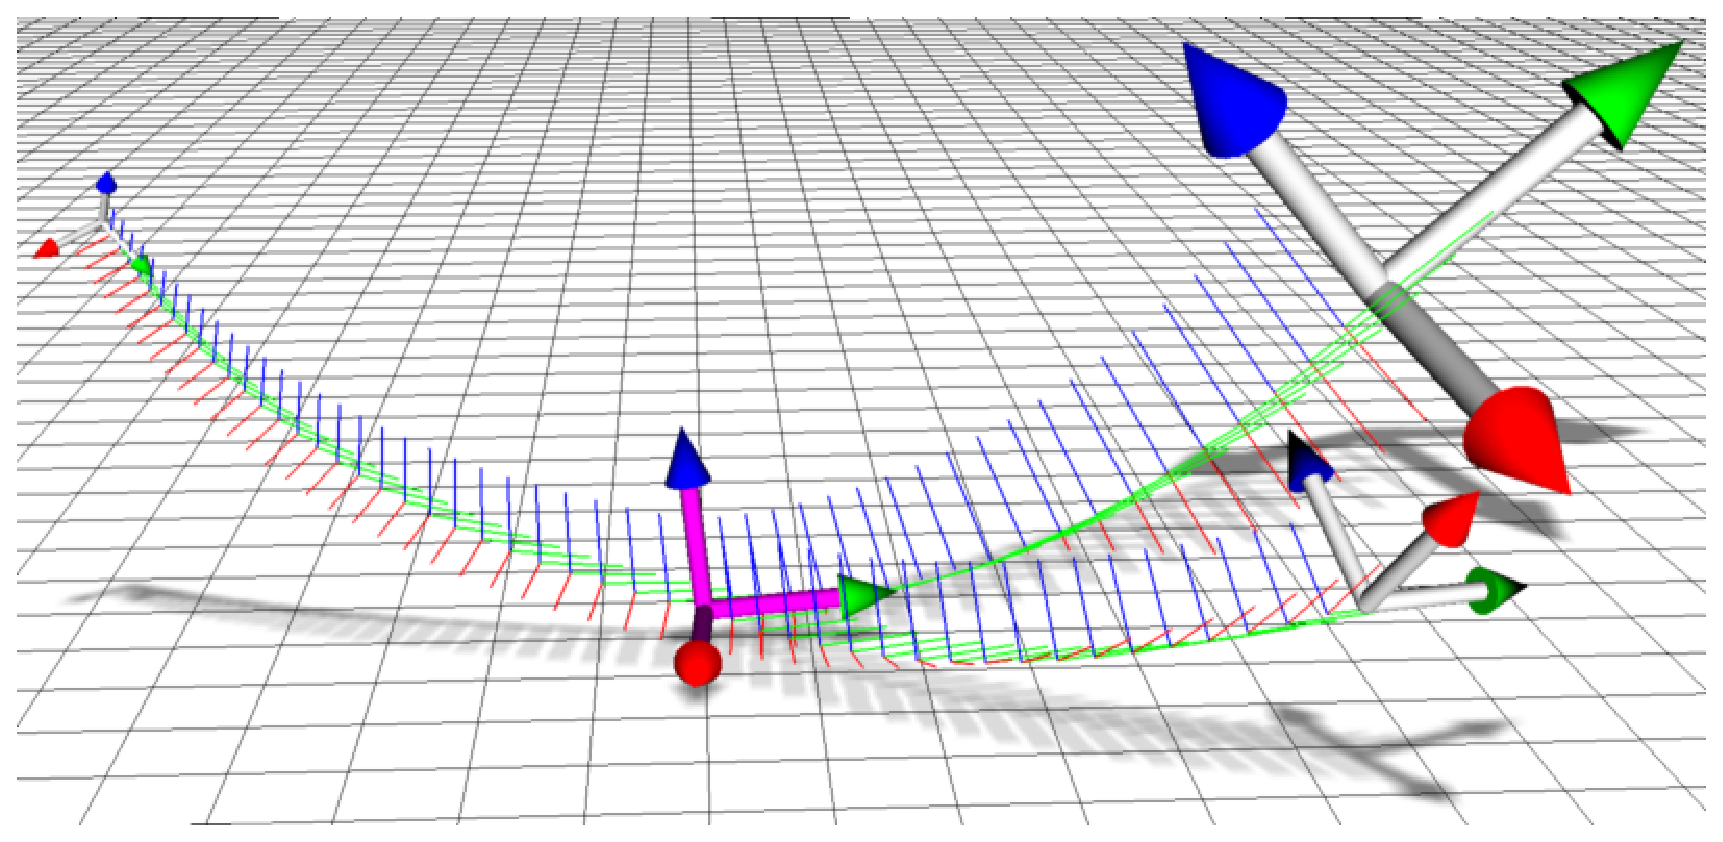
\includegraphics[width=0.95\linewidth]{egfigure.eps}
}

\end{center}
   \caption{\small Example of caption.  It is set in Roman so that mathematics (always set in Roman: $B \sin A = A \sin B$) may be included without an
   ugly clash.}
\label{fig:long}
\label{fig:onecol}
\end{figure}



%=========================================================================
\section{FORMATTING YOUR PAPER}

All text must be in a one-column format. The main title (on the first page) should begin 1.0 inch (2.54 cm) from the top edge of the page. The second and following pages should begin 1.0 inch (2.54 cm) from the top edge. On all pages, the bottom margin should be 1-1/8 inches (2.86 cm) from the bottom edge of the page for $8.5 \times 11$-inch paper; for A4 paper, approximately 1-5/8 inches (4.13 cm) from the bottom edge of the page.

%-------------------------------------------------------------------------
\subsection{Margins and Page Numbering}

All printed material, including text, illustrations, and charts, must be kept within a print area 6-7/8 inches (17.5 cm) wide by 8-7/8 inches (22.54 cm) high.

%-------------------------------------------------------------------------
\subsection{Type-style and Fonts}

Wherever Times is specified, Times Roman may also be used. If neither is available on your word processor, please use the font closest in appearance to Times to which you have access.

MAIN TITLE. Center the title 1-3/8 inches (3.49 cm) from the top edge of the first page. The title should be in Calibri 14-point, boldface capitalized type. A subtitle may be optionally included. Leave a blank line after the title.

AUTHOR NAME(s) and AFFILIATION(s) are to be centered beneath the title and printed in Times 11-point, non-boldface type. This information is to be followed by one blank line.

The ABSTRACT and MAIN TEXT are to be in a one-column format.

MAIN TEXT. Type main text in 11-point Times, single-spaced. Do NOT use double-spacing. All paragraphs should be indented 1 pica (approx. 1/6 inch or 0.422 cm). Make sure your text is fully justified---that is, flush left and flush right. Please do not place any additional blank lines between paragraphs.

Figure and table captions should be 10-point Roman type as in figure~\ref{fig:onecol}.  Short captions should be centered. 

Callouts should be 10-point Helvetica, non-boldface type.
Initially capitalize only the first word of section titles and first-,
second-, and third-order headings.

FIRST-ORDER HEADINGS. (For example, {\large \bf 1. INTRODUCTION}) should be Times 12-point boldface, capitalized, centered, with one blank line before, and one blank line after.

SECOND-ORDER HEADINGS. (For example, { \bf 1.1. Database elements}) should be Times 11-point boldface, initially capitalized, flush left, with one blank line before, and one after. If you require a third-order heading (we discourage it), use 10-point Times, boldface, initially capitalized, flush left, preceded by one blank line, followed by a period and your text on the same line.

If you know the Digital Object Identifier (DOI) number of your article, place it at the header of page 1 using Times 9-point type.

%-------------------------------------------------------------------------
\subsection{Footnotes}

Please use footnotes\footnote{This is what a footnote looks like.  It often distracts the reader from the main flow of the argument.} sparingly. Indeed, try to avoid footnotes altogether and include necessary peripheral observations in the text (within parentheses, if you prefer, as in this sentence).  If you wish to use a footnote, place it at the bottom of the column on the page on which it is referenced. Use Times 9-point type, single-spaced.

%-------------------------------------------------------------------------
\subsection{Program Code}

Program listings or program commands in the text are normally set in typewriter font, \eg, CMTT10 or Courier.

\noindent
{\it Example of a Computer Program}
\begin{verbatim}
program Inflation (Output)
  {Assuming annual inflation rates of 7%, 8%, and 10%,...
   years};
   const
     MaxYears = 10;
   var
     Year: 0..MaxYears;
     Factor1, Factor2, Factor3: Real;
   begin
     Year := 0;
     Factor1 := 1.0; Factor2 := 1.0; Factor3 := 1.0;
     WriteLn('Year  7% 8% 10%'); WriteLn;
     repeat
       Year := Year + 1;
       Factor1 := Factor1 * 1.07;
       Factor2 := Factor2 * 1.08;
       Factor3 := Factor3 * 1.10;
       WriteLn(Year:5,Factor1:7:3,Factor2:7:3,Factor3:7:3)
     until Year = MaxYears
end.
\end{verbatim}
%
\noindent
{\small (Example from Jensen K., Wirth N. (1991) Pascal user manual and
report. Springer, New York)}

%-------------------------------------------------------------------------
\subsection{References}

The heading of the References section must not be numbered. List and number all bibliographical references in 10-point Times, single-spaced, at the end of your paper. Please use regular and italic styles to distinguish different fields as shown in the References section. 

When referenced in the text, enclose the citation number in square brackets, for example~\cite{Alpher04}.  Where appropriate, include the name(s) of editors of referenced books. Please simply use the reference number, as in~\cite{Alpher04}.  Do not use ``Ref.~\cite{Alpher04}'' or ``Reference~\cite{Alpher04}'' except at the beginning of a sentence, e.g.  ``Reference~\cite{Alpher04} shows ...''. 

Examples of reference items of different categories shown in the References section include:
\begin{itemize}
\item Example of a book in~\cite{Arnold1989}
\item Example of a book in a series in~\cite{Santal'o1976}
\item Example of a journal article in~\cite{Alpher02}
\item Example of a conference paper in~\cite{Pham2011}
\item Example of a patent in~\cite{Pham2013}
\item Example of a web page in~\cite{Toshiba2011}
\item Example of a databook as manual in~\cite{Motorola1996}
\end{itemize}

\begin{table}
\begin{center}
\begin{tabular}{|l|c|}
\hline
Method & Frobnability \\
\hline\hline
Theirs & Frumpy \\
Yours & Frobbly \\
Ours & Makes one's heart Frob\\
\hline
\end{tabular}
\end{center}
\caption{\small Results.   Ours is better.}
\end{table}

%-------------------------------------------------------------------------
\subsection{Illustrations, graphs, and photographs}

All graphics should be centered with a minimum quality of 300 dpi (\ie 300 dots per inch).  Please ensure that any point you wish to make is resolvable in a printed copy of the paper.  Resize fonts in figures to match the font in the body text, and choose line widths which render effectively in print.  Many readers (and reviewers), even of an electronic copy, will choose to print your paper in order to read it.  You cannot insist that they do otherwise, and therefore must not assume that they can zoom in to see tiny details on a graphic.

When placing figures in \LaTeX, it's almost always best to use \verb+\includegraphics+, and to specify the  figure width as a multiple of the line width as in the example below
{\small\begin{verbatim}
   \usepackage[dvips]{graphicx} ...
   \includegraphics[width=0.8\linewidth]
                   {myfile.eps}
\end{verbatim}
}

%-------------------------------------------------------------------------
\subsection{Color}

Color is valuable, and will be visible to readers of the electronic copy.
However ensure that, when printed on a monochrome printer, no important
information is lost by the conversion to grayscale.

%=========================================================================
\section{CONCLUSIONS}

The paper ends with a conclusion.



%=========================================================================
\section*{APPENDIX}

Appendixes, if needed, appear before the acknowledgment.



%=========================================================================
\section*{ACKNOWLEDGMENT}

The preferred spelling of the word ``acknowledgment'' in American English is without an ``e'' after the ``g.'' Use the singular heading even if you have many acknowledgments. Avoid expressions such as ``One of us (S.B.A.) would like to thank ... .'' Instead, write ``F. A. Author thanks ... .'' In most cases, sponsor and financial support acknowledgments are placed in the unnumbered footnote on the first page, not here.



%=========================================================================
% References

% BibTeX users please use
{\small
\bibliographystyle{IEEEtranS} % sorted IEEE style
\bibliography{template} % name your BibTeX data base
}

%% Non-BibTeX users please use
%\begin{thebibliography}{}
%%
%% and use \bibitem to create references. Consult the Instructions
%% for authors for reference list style.
%%
%\bibitem{RefJ}
%% Format for Journal Reference
%Author, Article title, Journal, Volume, page numbers (year)
%% Format for books
%\bibitem{RefB}
%Author, Book title, page numbers. Publisher, place (year)
%% etc
%\end{thebibliography}

%=========================================================================
% Dates

%\hfill\it Nh\aang n b\ah i ng\ah y 20 - 12 - 2002

%\hfill Nh\aang n l\ang i sau s\uwhoi a ng\ah y 29 - 7 -2003

\hfill {\it Received on October 14 - 2003}

\hfill {\it Revised on January 14 - 2004}
\end{document}
